\documentclass[twocolumn]{article}
\usepackage{amsmath}
\usepackage{graphicx}
\graphicspath{documents/}
\usepackage{caption}
\captionsetup{font=scriptsize}
\usepackage[margin=0.5in]{geometry}

\title{Statistics, Uncertainties and Linear Fitting}
\author{Jorge A. Garcia}
\date{February 6th, 2018\\\line(1,0){500}}

\begin{document}
 \maketitle
 
 \section{Uncertainties}
 
 Diffraction equation:
 \begin{equation*}
  m\lambda = dsin\theta
 \end{equation*}
 Derivation of expression for $\Delta\lambda$:
 \begin{align*}
  (\Delta\lambda)^2 &= (\frac{1}{m} sin\theta)^2 (\Delta d)^2 + (\frac{1}{m} dcos\theta)^2 (\Delta\theta)^2 \\
  &= (\frac{1}{m})^2 (sin^2\theta (\Delta d)^2 + d^2 cos^2\theta (\Delta\theta)^2)
 \end{align*}
 \begin{equation*}
  \boxed{\Delta\lambda = \frac{1}{m} \sqrt{ sin^2\theta (\Delta d)^2 + d^2 cos^2\theta (\Delta\theta)^2 }}
 \end{equation*}
 Given the values:
 \begin{align*}
  m &= 1 \\
  d &= (600)^{-1} mm \\
  \Delta d/d &= 1\% \\
  \theta &= 15 deg \\
  \Delta\theta &= 0.5 deg
 \end{align*}
 Evaluation for $\lambda$:
 \begin{equation*}
  \lambda = \frac{dsin\theta}{m} = \frac{ [(600)^{-1} mm] sin (15 deg)}{1} \\
 \end{equation*}
  \begin{equation*}
  \boxed{\lambda = 4.3 \times 10^{-4} m = 430 \mu m}
 \end{equation*}
 Evaluation for $\Delta\lambda$:
 \begin{align*}
  \Delta\lambda &= \frac{1}{m} \sqrt{ sin^2\theta (\Delta d)^2 + d^2 cos^2\theta (\Delta\theta)^2} \\
  &= \frac{1}{1} \sqrt{ [sin^2(15 deg)] (\frac{1}{6000}m)^2 + (\frac{1}{600}m)^2 [cos^2(15 deg)] (0.5 deg)^2} \\
 \end{align*}
 \begin{equation*}
  \boxed{\Delta\lambda = 8.1 \times 10^{-4} m = 810 \mu m}
 \end{equation*}
 \vfill\eject % Breaks off columns
 \section{Linear Least Squares Fit}
 Having programmed an analysis routine on Python and plotting the data and fit, these are the results:
 \centerline{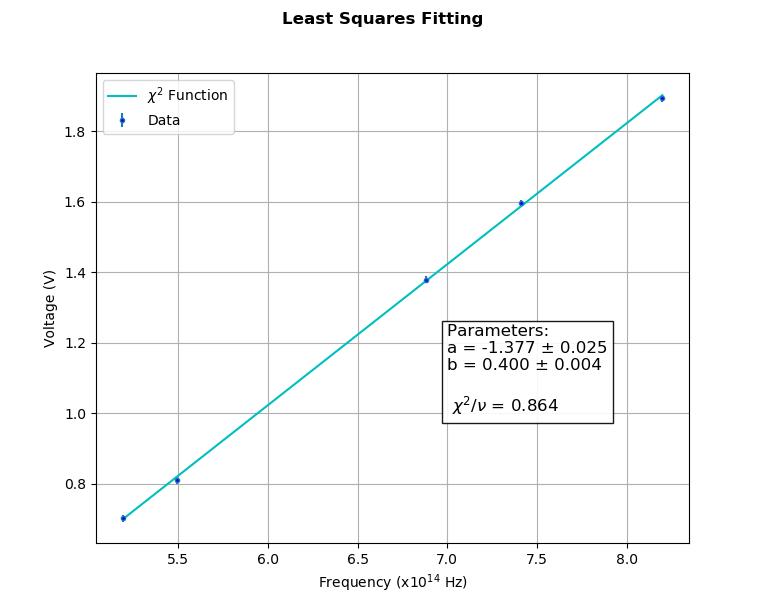
\includegraphics[scale = 0.6]{fig2}}
 The $\chi^2 / \nu$ is close to the ideal value of 1, so the linear fit is a good approximation to the system's function.
 \newpage
 \section{Geiger Counter - Radiation Decay}
 \subsection{Low Count-Rate Data}
 The mean number of counts $\bar{r}$, and the standard deviation $s$ without the radioactive sample is:
 \begin{align*}
 \bar{r} &= \frac{1}{N} \sum_{n=1}^{N} r_n = 1.92 \\
 s &= \sqrt{ \frac{1}{N-1}\sum_{r=1}^{N}(r - \bar{r})^2} = 1.37
 \end{align*}
 Since we are counting a random event, the data should follow a Poisson distribution. This means that the standard deviation squared should approximate the mean.
 Given our obtained data:
 \begin{equation*}
  s^2 = 1.87 \approx \bar{r} = 1.92 
 \end{equation*}
  The fraction of trials with an absolute deviation from the mean larger than the standard deviation $s$ is approximately $30\%$ of the sample. If one were to look at the
  probability of getting a result above that of the mean of the ideal Poisson distribution($\approx 2$), then:
 \begin{equation*}
  \sum_{r=3}^{5} P_\mu(r) = \sum_{r=3}^{5} \frac{\mu^re^{-\mu}}{r!} = 29\%
 \end{equation*}
 Giving indication that our results are very close to that of a Poisson distribution with the same mean.
 
 The following figure shows a histogram of the data taken, as well as calculated Poisson and Normal distributions from the data's parameters:
 \centerline{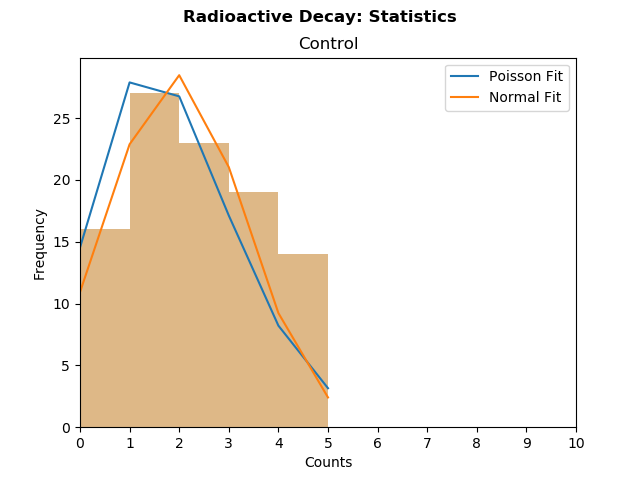
\includegraphics[scale = 0.6]{fig3a}}
 
 As can be seen, the Poisson distribution gives a much better model for the data, showing that the number of counts from the background detected by 
 the Geiger-Müller Counter is entirely random.
 \vfill\eject
 The following figure shows a plot of the data points of the experiment, displaying counts against sample number:
 \centerline{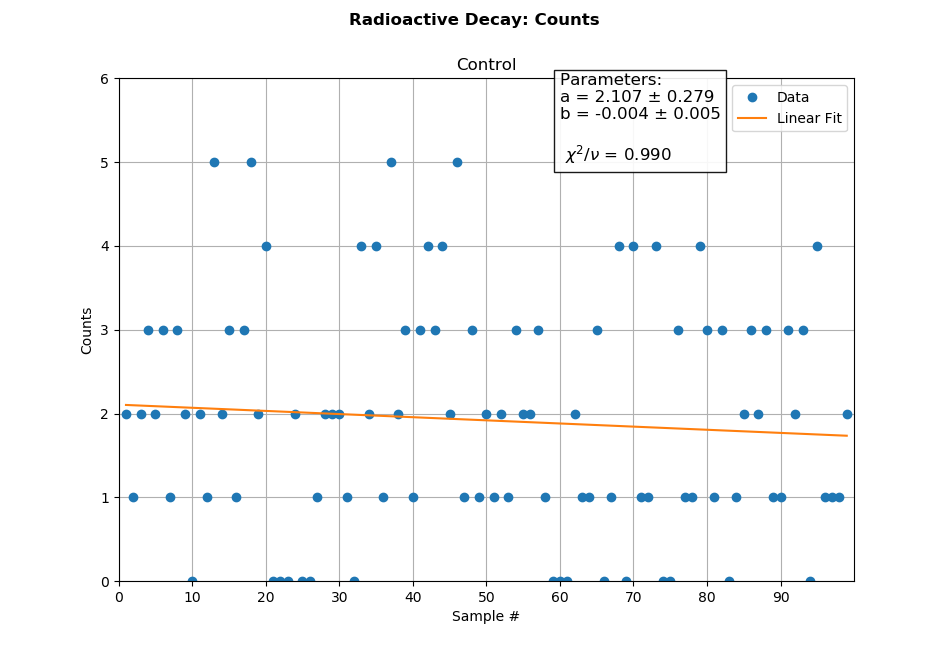
\includegraphics[scale = 0.41]{fig3b}}
 A linear Least Squares Fit was used in attempt to recreate the trend of the data. While the experiment assumed that the probability of detecting a
 radioactive decay product was constant in time ($a = \bar{r} = 1.92 , b = 0$), the calculated parameters were very close to the ideal values, within their uncertainties.
 Therefore, it can be assumed that the detection is constant throughout time.

 \subsection{High Count-Rate Data}
 The same process is used to analyze the high count-rate data, which includes the sample.
 
 The mean and the standard deviation of this set:
  \begin{align*}
 \bar{r} &= 54.23 \\
 s &= 9.09 \\
 s^2 = 82.54 &\neq \bar{r} = 54.23
 \end{align*}
 The comparison of the standard deviation and the mean means that this should not follow a Poisson distribution, since now there is a source of decay.
 
 The fraction of trials with an absolute deviation from the mean larger than the standard deviation $s$ is approximately $26\%$ of the sample. A Poisson
 distribution would expect to see:
 \begin{equation*}
  \sum_{r=55}^{92} P_\mu(r) = 48\%
 \end{equation*}
 There's a big discrepancy between both of these values as well.
 \newpage
 Plotting the histogram of the data and fitting both a Poisson and Normal distribution:
 \centerline{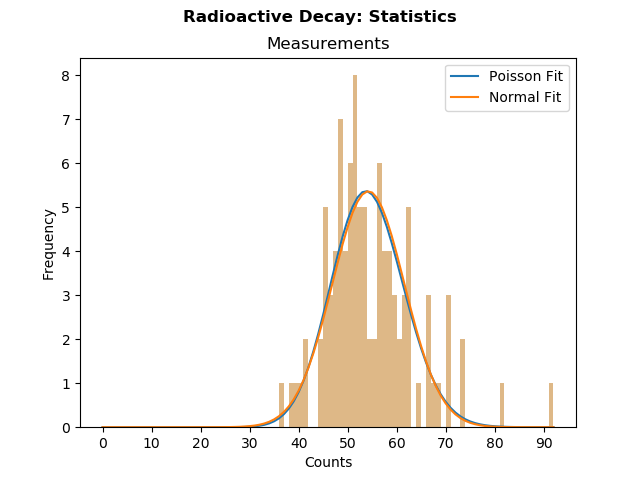
\includegraphics[scale = 0.6]{fig3c}}
 It can be seen that at this point the Poisson and Normal distributions are very similar, which makes sense since the Normal distribution is just a
 limiting case of the Poisson distribution ($\mu \gg 1$). Their numerical differences on the plot is due to how the Normal distribution is
 approximated, being:
 \begin{equation*}
  P(r) = \frac{1}{\sigma\sqrt{2\pi}} e^{-(r-\bar{r})^2 / 2\sigma^2}
 \end{equation*}
 While that of the Poisson distribution is:
 \begin{equation*}
  P(r) = \frac{\bar{r}^r e^{-\bar{r}}}{r!}
 \end{equation*}
  The following figure shows the plot of the data points of the experiment and its appropriate Linear Least Squares Fit as well:
 \centerline{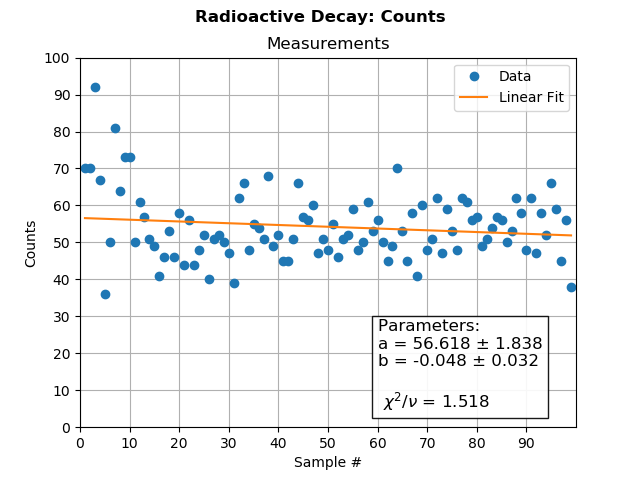
\includegraphics[scale = 0.6]{fig3d}}
 A good approximation is achieved, with the parameters being close to their expected values ($a = \bar{r} = 54.23, b = 0$).
 \vfill\eject
 \subsection{Determining the Source Count Rate}
 With the obtained data, the source's actual count rate can be determined. Knowing that:
 \begin{align*}
  R_{tot} = 
 \end{align*}

 
\end{document}